\clearpage{\pagestyle{empty}\cleardoublepage}
\chapter{Visualizzazione dati sull'utilizzo del progetto BolognaWiFi}
In questo capitolo andremo a trattare l'applicazione sviluppata, partendo da alcune considerazioni sui dati ufficiali forniti pubblicamente dal Comune di Bologna, per arrivare ad analizzare la struttura della stessa webapp.

Approfondiremo quindi i principali obiettivi, i problemi affrontati, le soluzioni implementate e l'ambiente di lavoro impiegato, per mostrare infine qualche schermata dell'applicazione così realizzata.

\section{Il caso studio: dati del BolognaWiFi}
% Descrizione del dataset, valore informativo, applicazioni per la pianificazione e gestione urbana
Il Comune di Bologna offre una serie di Open Data relativi al BolognaWiFi, riguardanti affollamento, affluenza e spostamenti, che vengono pubblicati ogni giorno mediante la rete Internet, in formato JSON. Il loro contenuto si riferisce a tutte le entrate giornaliere, riguardo alle varie zone e spostamenti, aggiornate a tre giorni prima della data odierna.

% Lo scopo della nostra applicazione è realizzare una visualizzazione dei dati in grado di mantenerne le informazioni sia a livello spaziale che temporale. Vedremo in seguito come siamo riusciti a sviluppare una tale dataviz e come il relativo sito degli Open Data non consenta una visualizzazione efficace dei dati.

Tutti questi dati sono stati aggregati in maniera oraria e anonima, quindi è impossibile risalire ai singoli dispositivi, rispettando così la privacy degli utenti. Tuttavia, la struttura dei dati non è omogenea in tutti e tre i dataset, quindi andremo a esplorarla nel dettaglio.

\subsection{Spostamenti}
Per gli spostamenti viene registrata una nuova entrata per ogni spostamento che viene effettuato in una data ora del giorno. Non è detto che ad ogni ora del giorno corrisponda almeno uno spostamento da una zona all'altra, in quanto non è detto che avvengano sempre, si pensi ad esempio durante le ore notturne.

\begin{figure}[H]
    \centering
    \includegraphics[width=0.75\textwidth]{spostamenti_alt}
    \caption[Struttura dei dati sugli spostamenti]{Dati relativi agli spostamenti, in formato JSON, riferiti ai movimenti da Parco del Cavaticcio a Mambo, alle ore 16 del 18 maggio 2021.}
    \label{fig:movements}
\end{figure}

Tali spostamenti sono direzionati, quindi uno spostamento dalla Biblioteca Salaborsa a Palazzo D'Accursio verrà registrato separatamente da quello effettuato, inversamente, da Palazzo D'Accursio a Biblioteca Salaborsa. Anche in questo caso, entrambe le direzioni degli spostamenti sono indipendenti l'una dall'altra, e non è detto che esistano entrambe in una certa ora. Per esempio, potremmo avere una direzione in cui si spostano 100 persone (o meglio, dispositivi), mentre nell'altra se ne spostano 0 o comunque una quantità trascurabile ai fini del rilevamento dati di BolognaWiFi, quindi in entrambi questi ultimi due casi non verrebbe creata nessuna nuova entrata sul database di Open Data. Questo aiuta anche a garantire la privacy degli utenti, in quanto se venissero pubblicati i dati di un singolo dispositivo in una certa direzione il diritto alla privacy potrebbe venire violato.

\subsection{Affollamento e Affluenza}
Dato che affollamento e affluenza contengono dati aventi una struttura molto simile tra loro, possiamo trattarli insieme. Per entrambi viene registrata una nuova entrata per ogni ora del giorno, in ciascuna zona di Bologna coperta dal servizio BolognaWiFi.

\begin{figure}[H]
    \centering
    \includegraphics[width=0.75\textwidth]{affollamento_alt}
    \caption[Struttura dei dati sull'affollamento]{Dati riguardanti l'affollamento, in formato JSON, riferiti a Piazza Malpighi alle ore 20 del 12 febbraio 2024. Notare l'attributo \textit{ora} che viene incluso nel timestamp di \textit{data} in fuso orario UTC.}
    \label{fig:crowding}
\end{figure}

\begin{figure}[H]
    \centering
    \includegraphics[width=0.75\textwidth]{affluenza_alt}
    \caption[Struttura dei dati sull'affluenza]{Dati riguardanti l'affluenza, in formato JSON, riferiti al Museo della Musica, alle ore 23 del 27 febbraio 2024. Notare l'attributo \textit{ora} che viene incluso nel timestamp di \textit{data} in fuso orario UTC.}
    \label{fig:attendance}
\end{figure}

\section{Struttura del database}
La struttura dei dati ottenuti dall'interrogazione delle API, così come possiamo vedere in Figura~\ref{fig:movements}, Figura~\ref{fig:crowding} e Figura~\ref{fig:attendance}, è abbastanza semplice di per sé. Tuttavia, tale semplicità nasconde dei problemi di gestione delle ridondanze quando vengono salvati i dati su database, ciò avviene per svariati motivi che ora approfondiremo.

\subsection{Aree}
Innanzitutto, le informazioni relative alle aree e coordinate sono salvate in maniera differente nei tre dataset. Negli spostamenti si collegano solo i nomi e gli identificatori di ciascuna area attinente al vettore movimento, mentre sia in affollamento che in affluenza vengono specificate anche le relative coordinate del poligono, insieme a quelle del suo centroide.

Questo comporta fin da subito la necessità di creare un'entità per le aree e una separata per ciascuna coordinata, in quanto ogni poligono ha un numero variabile di punti. In questo modo non solo rimuoviamo la ridondanza tra affollamento e affluenza, ma permettiamo anche di collegare due poligoni a ciascuno spostamento, uno di partenza e uno di arrivo, cosa che non sarebbe possibile se non avessimo aggregato i tre dataset.

Notiamo subito che tale accortezza è possible solamente perché tutti e tre i dataset afferiscono alle stesse aree, ovvero i poligoni, delimitati dalla copertura del segnale di BolognaWiFi, quindi il loro dominio delle aree è completamente sovrapponibile.

\subsection{Spostamenti}
In questo modo, abbiamo assegnato un poligono di partenza e uno di arrivo a ciascuno spostamento. Rimane tuttavia il fatto che esista un numero \( n \) di spostamenti giornalieri, con \( n \leq 24 \), quindi al momento avremmo un numero esageratamente alto di entrate su database, che diventerebbe un problema in termini di richieste al server per visualizzare i dati giornalieri.

Questo problema può essere efficacemente risolto aggregando tutti i dati giornalieri: per fare ciò, fissata un'area di partenza e una di arrivo per una precisa data, creiamo 24 colonne per l'attributo \textit{percentile\_50} e altrettante 24 per \textit{tot\_pass}. In questo modo ottimizziamo il recupero dei dati effettuato dal client mediante richieste server, riducendo il numero di chiamate fino a 24 volte: basta semplicemente scaricare tutti i dati di un giorno, e utilizzarli fino a quando l'utente non chiama i dati di un altro giorno.

Riguardo al significato degli attributi, \textit{tot\_pass} è il numero di passeggeri che transitano da una zona A a una zona B nell'arco di un'ora in un determinato giorno. Invece, \textit{percentile\_50} è il mediano di tutti i \textit{tot\_pass} calcolati per tutti i giorni a una determinata ora, fino al giorno in cui vengono salvati i dati sul database di Open Data.

In questo caso, l'aggregazione dei dati è semplice perché nel dataset, nessun giorno ha un numero di entrate superiore a 24, cosa non scontata considerando che il cambio dell'ora genera un giorno con 23 ore in primavera e uno con 25 in autunno. Tale affermazione è affidabile in quanto la registrazione dei dati sugli spostamenti è cominciata l'1 aprile 2021.

\subsection{Affollamento e Affluenza}
Ancora una volta, questi due dataset si rivelano simili: avendo un insieme di attributi molto simili e lo stesso set di coordinate dei poligoni, basta scegliere uno qualunque dei due dataset per popolare le tabelle di area e coordinate che abbiamo visto prima.

In questo modo, entrambe le sezioni di \textit{geo\_shape} e \textit{geo\_point\_2d} vengono assorbite in area e coordinate, alleggerendo la struttura delle tabelle di affollamento e affluenza che andremo a realizzare. Possiamo notare che tutti i dati relativi ad affollamento e affluenza hanno un \textit{"type": "Feature"} e \textit{"type": "Polygon"}, che possono essere tranquillamente ignorati essendo uguali in tutto il dataset.

Anche qui, per ottimizzare le richieste al server nello stesso modo che abbiamo visto per gli spostamenti, aggreghiamo le 24 ore dello stesso giorno all'interno della stessa entrata, ma non solo: data la loro somiglianza, affollamento e affluenza possono essere aggregati all'interno della stessa tabella. Questo è possibile perché entrambe le loro entrate riguardano tutte le aree di Bologna ad ogni ora del giorno, quindi il numero totale è sempre uguale.

Tuttavia, in questo caso in entrambi i dataset vi sono giorni con 23 o 25 entrate giornaliere, a causa del cambio dell'ora. Tale problema si risolve facilmente, considerando che tutti gli eccessi hanno valori nulli: in caso di conflitto, basta tenere il valore massimo, in quanto uno dei due è per forza zero, mentre in caso di deficit basta assegnare 0 come valore al dato mancante.

Inoltre, sorge un ulteriore problema iniziale dovuto al fatto che i dati di affluenza sono disponibili a partire dal 1 gennaio 2024, mentre quelli riguardanti l'affollamento cominciano dal 15 gennaio 2024. Ancora una volta si risolve semplicemente assegnando uno 0 ai valori mancanti, ovvero a tutti quelli nelle due settimane in cui non vi sono dati riguardanti l'affollamento.

\subsection{Schema finale}
Dopo tutte le precedenti considerazioni, riportiamo in Figura~\ref{fig:database} lo schema finale del database. Per evitare di ottenere un database enorme in termini di spazio su disco, abbiamo prestato particolare attenzione ad utilizzare la quantità di memoria minore possibile per ogni attributo delle tabelle.

In particolare, considerando che gli spostamenti (sia totali che mediani), l'affollamento e l'affluenza orari raggiungono valori sempre interi che non superano mai la quantità di 10~000 e non sono mai inferiori a zero. Di conseguenza, possiamo utilizzare un tipo di dato \textit{unsigned short} senza avere timori relativi ad un possibile overflow, anzi possiamo mantenere pure una certa quantità di margine, occupando solo 2 bytes per numero, dimezzando lo spazio richiesto in confronto ai 4 bytes occupati da un normale \textit{unsigned int}.

Inoltre, una simile considerazione può essere effettuata per i numeri decimali relativi alle coordinate dei punti dei poligoni, in quanto vi sono sempre due cifre intere e 14 o 15 cifre decimali. Riguardo alle due cifre intere, possiamo utilizzarne sempre due solamente considerando la posizione geografica di Bologna, in quanto se la latitudine non rappresenta un problema, la longitudine talvolta può assumere valori a tre cifre intere in base alla posizione sulla Terra. In questo modo, su MySQL gli viene assegnato il tipo di dato \textit{decimal(17,15)}, con 15 cifre decimali su 17 cifre totali, escludendo la virgola.

\begin{figure}[H]
    \centering
    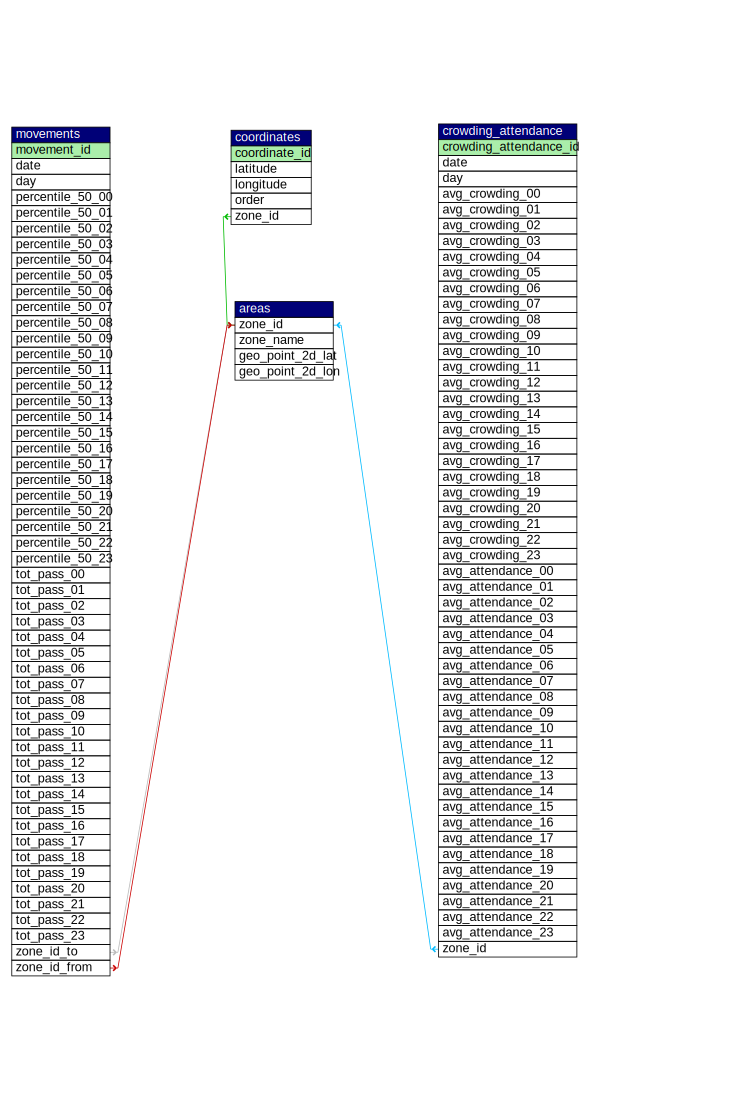
\includegraphics[width=\textwidth]{database.png}
    \caption[Schema del database]{Schema del database di BolognaWiFiMap. Notare la lista di attributi definiti per ciascuna ora.}
    \label{fig:database}
\end{figure}

\section{Connessione tra frontend e backend}
Dopo aver installato Vue.js e creato il progetto utilizzando Vite, ovvero un plugin di Vue per la nuova sintassi SFC (Single-File Components), abbiamo impostato l'indirizzo e la porta del server nel file di configurazione \Verb_vite.config.js_, settandolo a 0.0.0.0 per permettere al frontend di comunicare col backend indipendentemente dall'indirizzo del server, che in questo caso si riferisce a quello del server Apache. Inoltre, abbiamo specificato l'alias \Verb_@_ per definire la directory \Verb_./src/frontend_, semplificando il percorso dei file da importare.

\begin{figure}[H]
    \centering
    \includegraphics[width=\textwidth]{vite_config}
    \caption[Configurazione delle impostazioni Vite]{Configurazione delle impostazioni Vite relative al progetto Vue, dove si definiscono in particolare l'indirizzo e la porta per accedere al server.}
    \label{fig:vite_config}
\end{figure}

\section{Single-Page App}
Questa applicazione è stata realizzata seguendo il modello della \textit{Single-Page App}, ovvero una sola pagina web che carica selettivamente i suoi componenti o aggiorna i suoi dati senza necessità di ricaricare la pagina. Questo è permesso sia dallo stesso framework Vue.js, sia dall'implementazione di richieste AJAX che il client effettua al server.

\section{Implementazione richieste AJAX}
Le richieste AJAX sono effettuate in modo asincrono dal client al server per ottenere dei dati che verranno utilizzati per aggiornare la pagina, evitando di dover effettuare un ricaricamento della stessa. Per la sua implementazione abbiamo utilizzato la funzione \Verb_fetch()_ built-in di JavaScript, creando tre funzioni per aggiornare rispettivamente le aree, con \Verb_fetchAreas()_, gli spostamenti, con \Verb_fetchMovements()_, e infine l'affollamento insieme all'affluenza, con \Verb_fetchCrowdingAttendance()_. 

Abbiamo definito tutte queste funzioni nel file \Verb_api.js_, essendo molto semplici riportiamo in Figura~\ref{fig:ajax_api_movements} solo quella relativa agli spostamenti. In particolare, queste custom API utilizzano l'indirizzo corrente comprensivo di porta, per poi appendere a tale stringa l'url specifico dell'API a cui si vuole effettuare la richiesta. Si noti come questo setup presuppone un deployment di frontend e backend sullo stesso server, o quantomeno di un ridirezionamento tramite proxy di tali richieste effettuate a frontend verso l'url appropriato del backend, se dovessero essere in deployment su server diversi.

\begin{figure}[H]
    \centering
    \includegraphics[width=\textwidth]{ajax_api_movements}
    \caption[Funzione AJAX per ottenere la lista dei movimenti di una specifica data]{Implementazione di una funzione che effettua una richiesta AJAX per ottenere la lista dei movimenti di una specifica data.}
    \label{fig:ajax_api_movements}
\end{figure}

\section{Popolamento del database}
Affinché le richieste AJAX possano andare a buon fine, bisogna aver popolato il database. Questo compito è svolto mediante l'esecuzione del file \Verb_updater.php_, il quale controlla l'ultima data dei dati raccolti sul database e provvede ad aggiornarli, scaricando tutti i nuovi dati.

In fase di development o test, questo script viene lanciato manualmente, ma in un futuro deployment basterebbe automatizzare la sua esecuzione utilizzando Task Scheduler su Windows o un Cron Job su Linux. Tale script, riportato in Figura~\ref{fig:updater} richiama 3 funzioni differenti per svolgere il suo compito, che qui non mostreremo per via della loro lunghezza.

\begin{figure}[H]
    \centering
    \includegraphics[width=\textwidth]{updater_noligature}
    \caption[]{Script che viene eseguito per effettuare il setup o per aggiornare i dati sul database, utilizzando gli url definiti in \textit{urls.json} per effettuare le chiamate alle API del sito degli Open Data di BolognaWiFi \cite{BolognaWiFi_Spostamenti,BolognaWiFi_Affollamento,BolognaWiFi_Affluenza}.}
    \label{fig:updater}
\end{figure}

Innanzitutto, viene aggiornata la lista delle aree, nel caso se ne trovino di nuove. Quindi si scaricano, in ordine, prima i movimenti, poi l'affollamento insieme all'affluenza. All'interno di entrambe le funzioni, vengono scaricati i dati giorno per giorno, fino ad arrivare agli ultimi disponibili. Tuttavia, date le limitazioni delle API offerte da BolognaWiFi, vengono scaricati al massimo 100 elementi alla volta. Questo chunk così ottenuto viene messo in coda in una lista, per poi effettuare una nuova chiamata alla stessa API riguardante lo stesso giorno, ma con un offset aumentato di 100. Le stesse API pongono un limite totale di 10~100 alla somma di offset e numero di elementi, ma considerando che in un singolo giorno non si arriva nemmeno a 2~000 elementi totali in tutti e tre i dataset, tale limite effettivo di 10~000 all'offset non è poi così restrittivo.

% \section{Funzionalità}
\section{Informazioni su una zona o spostamento}
\section{Calcolo del colore di una zona}
\section{Raggruppamento dei dati giornalieri}
\section{Questionario SUS sull'esperienza utente}